\chapter{Introduction}
\label{chapter:introduction}

As neuromorphic computing becomes more popular, various  applications for such systems emerge and make use of analogue hardware's advantages over traditional computers \reference{paper on future of neuromorphic computing}.
But to do so, one must be familiar with the system that is used as it often differs in many ways from common computer architectures.
Thus programing for such systems can feel odd at times as users need to abandon some familiar techniques and acquire new skills instead.
This is a hurdle for many users when developing new experiments and initially takes a significant amount of time. 

The more a system abandons common elements of programming which users are accustomed to the more problems can emerge from this.
Not only will fewer users take the initiative of writing for such systems but also can code easily get confusing, hard to debug and at worst even ineffective.
\\
\\
An example of this is the current way of programming for the plasticity processing unit of the HICANN-DLS. 
It is responsible for applying so called plasticity rules to the neuromorphic system and resembles a commonly known processor which was modified for this cause.
Despite basic programming still being the same for this processor it differs for creating mentioned plasticity rules.
Although these are still programmed in a C environment, a user is given a set of functions and predefined macros that are based on low-level programming.

This was done to include users who want to write programs for the PPU despite being unfamiliar with low-level languages and leads to PPU programs having a distinct look and feel that is only in some regards similar to C.
Instead it is like pushing the user back to the origins of computing; for example reading out the value of a variable in memory needs unhandy workarounds and a repetitive set of code instructions.
\\
\\
The main reason we may feel reluctant to such outdated programming are the advantages of compilers, which became a standard for programmers over decades.

From the early stages of computing, compilers have developed towards a standard tool in everyday programming but at the same time became more of a black box that transforms a program into an executable file.
For this reason it may be difficult for some users to abandon such convenience and go back to low-level programming.

Luckily the PPU is not completely without compiler support as basic computing is supported but distinct features of the PPU are only usable on a low level.
This can easily cause inconvenience for users as these features are necessary to implement learning rules for synapses which are themselves elementary to neuromorphic programming.
As of now users need to repeatedly mix high-level with low-level programming when developing for the PPU which may lead to different problems as users have to adapt to this atypical style of programming.
At worst this can even lead to ineffective programs --- as performance is important for neuromorphic programming and the main advantage of the PPU --- and an unreasonable amount of time and work to achieve simple results.
\\
\begin{wrapfigure}{R}{0.4\textwidth}
    \centering
    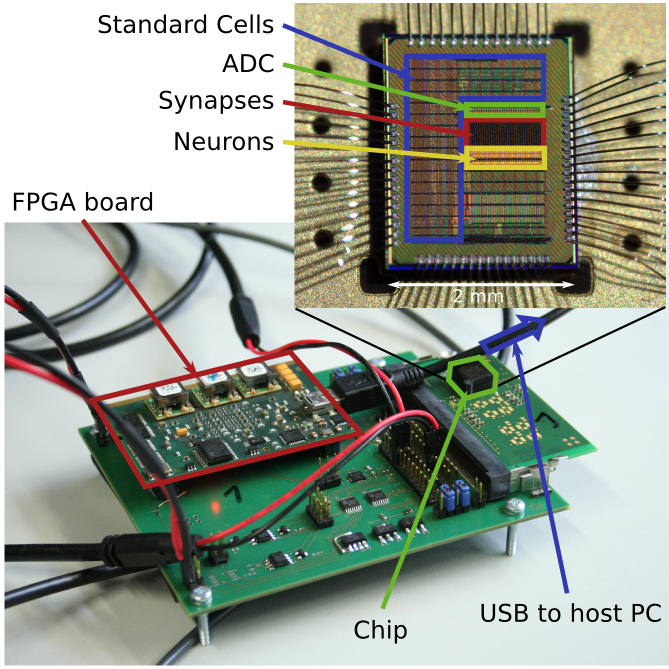
\includegraphics[width=0.4\textwidth]{pictures/Fig1.png}
    \caption{\label{fig:dlsboard} set-up of a HICANN-DLS test system}
\end{wrapfigure}
\\
This makes it obvious that compiler support is desirable as the PPU is yet not fully supported by any compiler.
Especially as compilers offer a convenient way of supporting various high-level programming languages.

The reason the PPU does not have compiler support is the custom nature of the processor architecture, which was developed solely for the BrainScaleS system and the HICANN-DLS.
It can be classified as an application specific instruction set architecture which is an intermediate form between general purpose processors and application specific integrated circuits and offers a partly customized instruction set that is optimized for certain applications.

With and without the help of the PPU the HICANN-DLS already is a platform for many interesting experiments that were conducted or are yet to be conducted in the near future.
Applications like in-the-loop training or RSTDP have been developed by various users despite the problem of low-level coding by either not using the PPU at all or acknowledging the low-level nature of the PPU and learning how to write programs that involve the PPU.
Even when taking the effort of learning to code for the PPU, users are constantly challenged by missing capabilities of program code such as creating parameterized functions which leads to repetitive code or difficulties when involving calibration into code.

As we do not want the PPU to be abandoned because of this, even though there is much potential to it, as a hand full of users continuously shows, users should be encouraged to develop applications for the PPU.
One way to do so is offering more tools that increase the capabilities of programs while at the same time reducing the effort it takes to develop for the PPU.
Besides achieving full high-level programming when working with the PPU, compiler support could also include code optimization and debugging features that help creating more applications like the above.
This work therefore aims to achieve compiler support of the PPU's hardware with as many features as possible and simplify programming for existing users what could also advertise the platform to new users and possibly accelerate performance of programs on the PPU.
At some point compiler support could also facilitate automatic code generation as a prerequisite for implementation of very high-level languages.
That would mean that users do not need to code for the PPU itself but instead create plasticity rules in existing program environments from where code is translated into PPU programs.
This creates also the need for optimization of PPU code which could be done by developers specifically for the PPU but it is far easier and likely more efficient to utilize existing optimization techniques that are built into virtually every compiler.
\\
\\
This thesis will focus on achieving aforementioned compiler support and briefly explain the process itself.
As fundamental knowledge of both processors and compilers is needed along the way the second chapter will start with a very basic introduction to both topics and go into detail for the processor and compiler that were used in this thesis.
This may not render additional literature obsolete but should explain the basic concepts to an extend which is sufficient.
Afterwards the process of extending the compiler is explained into some detail and the result as well as first test cases are presented.
The thesis will conclude in a resume and give an outlook to future applications and development of the compiler and the PPU.

Ultimately we want simplify to PPU programming overall and give users tools at hand that allow for many interesting experiments and encourage further development of the whole system.




